% !TEX encoding = UTF-8 Unicode
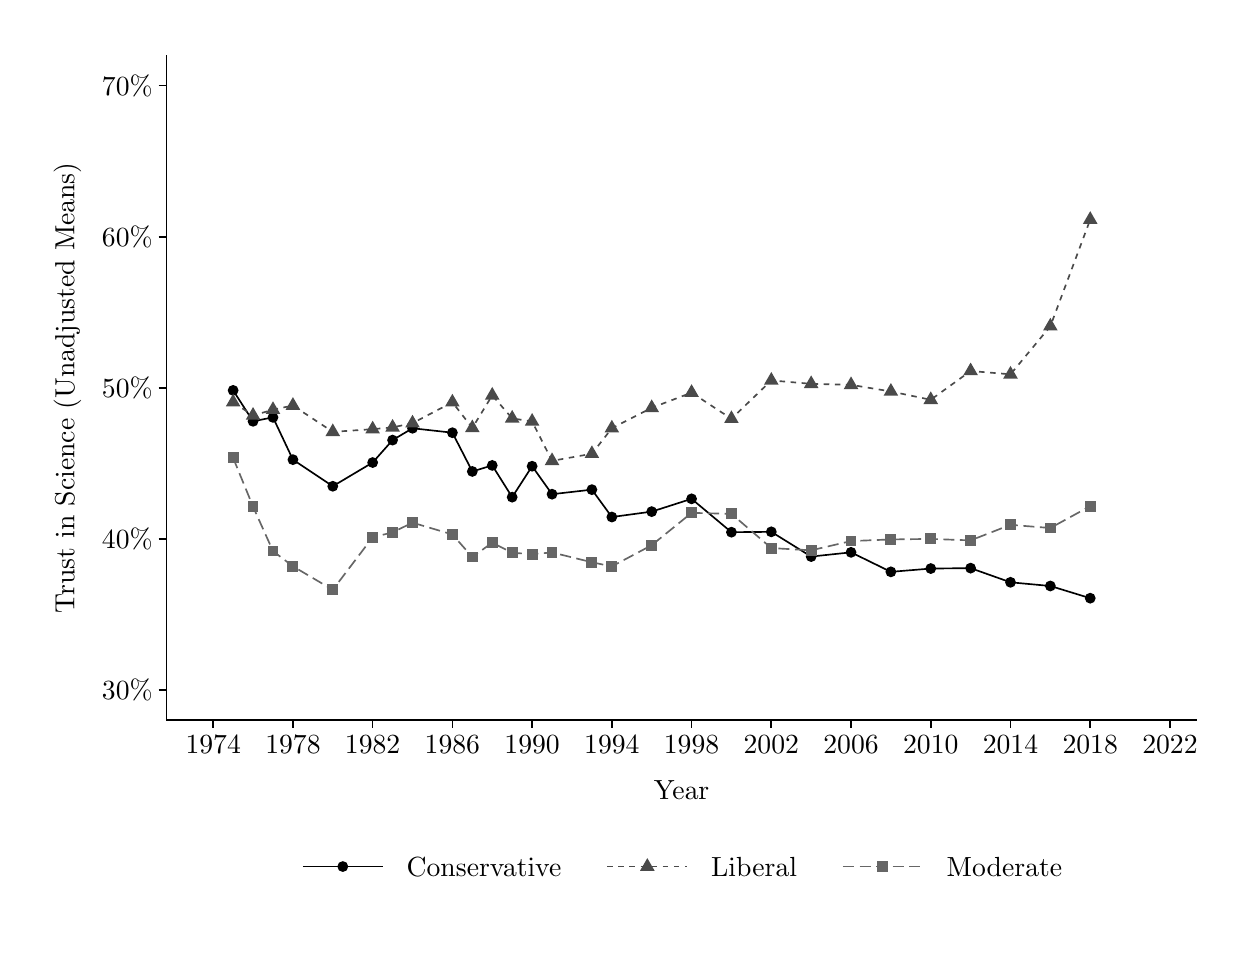
\begin{tikzpicture}[x=1pt,y=1pt]
\definecolor{fillColor}{RGB}{255,255,255}
\path[use as bounding box,fill=fillColor,fill opacity=0.00] (0,0) rectangle (432.48,324.36);
\begin{scope}
\path[clip] (  0.00,  0.00) rectangle (432.48,324.36);
\definecolor{fillColor}{RGB}{255,255,255}

\path[fill=fillColor] ( -0.00,  0.00) rectangle (432.48,324.36);
\end{scope}
\begin{scope}
\path[clip] ( 50.11, 74.07) rectangle (422.48,314.36);
\definecolor{fillColor}{RGB}{255,255,255}

\path[fill=fillColor] ( 50.11, 74.07) rectangle (422.48,314.36);
\definecolor{drawColor}{RGB}{0,0,0}

\path[draw=drawColor,line width= 0.6pt,line join=round] ( 74.24,193.29) --
	( 81.44,182.12) --
	( 88.64,183.54) --
	( 95.85,168.26) --
	(110.25,158.65) --
	(124.66,167.22) --
	(131.86,175.33) --
	(139.06,179.60) --
	(153.47,178.00) --
	(160.67,164.00) --
	(167.87,166.18) --
	(175.07,154.71) --
	(182.28,165.89) --
	(189.48,155.78) --
	(203.88,157.42) --
	(211.09,147.53) --
	(225.49,149.48) --
	(239.90,154.10) --
	(254.30,142.05) --
	(268.71,142.18) --
	(283.11,133.24) --
	(297.52,134.77) --
	(311.92,127.72) --
	(326.33,128.91) --
	(340.73,129.06) --
	(355.14,123.94) --
	(369.54,122.61) --
	(383.95,118.20);
\definecolor{drawColor}{gray}{0.29}

\path[draw=drawColor,line width= 0.6pt,dash pattern=on 2pt off 2pt ,line join=round] ( 74.24,189.03) --
	( 81.44,184.23) --
	( 88.64,186.31) --
	( 95.85,187.82) --
	(110.25,178.30) --
	(124.66,179.28) --
	(131.86,179.93) --
	(139.06,181.43) --
	(153.47,189.01) --
	(160.67,179.73) --
	(167.87,191.49) --
	(175.07,183.18) --
	(182.28,182.06) --
	(189.48,167.83) --
	(203.88,170.39) --
	(211.09,179.61) --
	(225.49,186.99) --
	(239.90,192.48) --
	(254.30,183.03) --
	(268.71,196.89) --
	(283.11,195.66) --
	(297.52,195.29) --
	(311.92,192.90) --
	(326.33,189.90) --
	(340.73,200.30) --
	(355.14,199.09) --
	(369.54,216.46) --
	(383.95,255.00);
\definecolor{drawColor}{gray}{0.40}

\path[draw=drawColor,line width= 0.6pt,dash pattern=on 4pt off 2pt ,line join=round] ( 74.24,168.91) --
	( 81.44,151.28) --
	( 88.64,135.23) --
	( 95.85,129.72) --
	(110.25,121.24) --
	(124.66,140.21) --
	(131.86,141.99) --
	(139.06,145.49) --
	(153.47,141.23) --
	(160.67,133.07) --
	(167.87,138.26) --
	(175.07,134.61) --
	(182.28,134.12) --
	(189.48,134.73) --
	(203.88,131.18) --
	(211.09,129.68) --
	(225.49,137.35) --
	(239.90,149.03) --
	(254.30,148.68) --
	(268.71,136.31) --
	(283.11,135.50) --
	(297.52,138.84) --
	(311.92,139.43) --
	(326.33,139.62) --
	(340.73,139.09) --
	(355.14,144.71) --
	(369.54,143.56) --
	(383.95,151.46);
\definecolor{fillColor}{RGB}{0,0,0}

\path[fill=fillColor] ( 74.24,193.29) circle (  1.96);
\definecolor{fillColor}{gray}{0.29}

\path[fill=fillColor] ( 74.24,192.08) --
	( 76.88,187.50) --
	( 71.60,187.50) --
	cycle;
\definecolor{fillColor}{gray}{0.40}

\path[fill=fillColor] ( 72.28,166.95) --
	( 76.20,166.95) --
	( 76.20,170.87) --
	( 72.28,170.87) --
	cycle;
\definecolor{fillColor}{RGB}{0,0,0}

\path[fill=fillColor] ( 81.44,182.12) circle (  1.96);
\definecolor{fillColor}{gray}{0.29}

\path[fill=fillColor] ( 81.44,187.28) --
	( 84.08,182.70) --
	( 78.80,182.70) --
	cycle;
\definecolor{fillColor}{gray}{0.40}

\path[fill=fillColor] ( 79.48,149.31) --
	( 83.40,149.31) --
	( 83.40,153.24) --
	( 79.48,153.24) --
	cycle;
\definecolor{fillColor}{RGB}{0,0,0}

\path[fill=fillColor] ( 88.64,183.54) circle (  1.96);
\definecolor{fillColor}{gray}{0.29}

\path[fill=fillColor] ( 88.64,189.36) --
	( 91.29,184.78) --
	( 86.00,184.78) --
	cycle;
\definecolor{fillColor}{gray}{0.40}

\path[fill=fillColor] ( 86.68,133.27) --
	( 90.61,133.27) --
	( 90.61,137.19) --
	( 86.68,137.19) --
	cycle;
\definecolor{fillColor}{RGB}{0,0,0}

\path[fill=fillColor] ( 95.85,168.26) circle (  1.96);
\definecolor{fillColor}{gray}{0.29}

\path[fill=fillColor] ( 95.85,190.87) --
	( 98.49,186.29) --
	( 93.20,186.29) --
	cycle;
\definecolor{fillColor}{gray}{0.40}

\path[fill=fillColor] ( 93.88,127.75) --
	( 97.81,127.75) --
	( 97.81,131.68) --
	( 93.88,131.68) --
	cycle;
\definecolor{fillColor}{RGB}{0,0,0}

\path[fill=fillColor] (110.25,158.65) circle (  1.96);
\definecolor{fillColor}{gray}{0.29}

\path[fill=fillColor] (110.25,181.35) --
	(112.89,176.78) --
	(107.61,176.78) --
	cycle;
\definecolor{fillColor}{gray}{0.40}

\path[fill=fillColor] (108.29,119.28) --
	(112.21,119.28) --
	(112.21,123.20) --
	(108.29,123.20) --
	cycle;
\definecolor{fillColor}{RGB}{0,0,0}

\path[fill=fillColor] (124.66,167.22) circle (  1.96);
\definecolor{fillColor}{gray}{0.29}

\path[fill=fillColor] (124.66,182.33) --
	(127.30,177.75) --
	(122.01,177.75) --
	cycle;
\definecolor{fillColor}{gray}{0.40}

\path[fill=fillColor] (122.69,138.24) --
	(126.62,138.24) --
	(126.62,142.17) --
	(122.69,142.17) --
	cycle;
\definecolor{fillColor}{RGB}{0,0,0}

\path[fill=fillColor] (131.86,175.33) circle (  1.96);
\definecolor{fillColor}{gray}{0.29}

\path[fill=fillColor] (131.86,182.98) --
	(134.50,178.40) --
	(129.22,178.40) --
	cycle;
\definecolor{fillColor}{gray}{0.40}

\path[fill=fillColor] (129.90,140.03) --
	(133.82,140.03) --
	(133.82,143.95) --
	(129.90,143.95) --
	cycle;
\definecolor{fillColor}{RGB}{0,0,0}

\path[fill=fillColor] (139.06,179.60) circle (  1.96);
\definecolor{fillColor}{gray}{0.29}

\path[fill=fillColor] (139.06,184.48) --
	(141.70,179.90) --
	(136.42,179.90) --
	cycle;
\definecolor{fillColor}{gray}{0.40}

\path[fill=fillColor] (137.10,143.53) --
	(141.02,143.53) --
	(141.02,147.45) --
	(137.10,147.45) --
	cycle;
\definecolor{fillColor}{RGB}{0,0,0}

\path[fill=fillColor] (153.47,178.00) circle (  1.96);
\definecolor{fillColor}{gray}{0.29}

\path[fill=fillColor] (153.47,192.06) --
	(156.11,187.48) --
	(150.82,187.48) --
	cycle;
\definecolor{fillColor}{gray}{0.40}

\path[fill=fillColor] (151.50,139.26) --
	(155.43,139.26) --
	(155.43,143.19) --
	(151.50,143.19) --
	cycle;
\definecolor{fillColor}{RGB}{0,0,0}

\path[fill=fillColor] (160.67,164.00) circle (  1.96);
\definecolor{fillColor}{gray}{0.29}

\path[fill=fillColor] (160.67,182.78) --
	(163.31,178.20) --
	(158.03,178.20) --
	cycle;
\definecolor{fillColor}{gray}{0.40}

\path[fill=fillColor] (158.71,131.11) --
	(162.63,131.11) --
	(162.63,135.03) --
	(158.71,135.03) --
	cycle;
\definecolor{fillColor}{RGB}{0,0,0}

\path[fill=fillColor] (167.87,166.18) circle (  1.96);
\definecolor{fillColor}{gray}{0.29}

\path[fill=fillColor] (167.87,194.54) --
	(170.51,189.96) --
	(165.23,189.96) --
	cycle;
\definecolor{fillColor}{gray}{0.40}

\path[fill=fillColor] (165.91,136.30) --
	(169.83,136.30) --
	(169.83,140.23) --
	(165.91,140.23) --
	cycle;
\definecolor{fillColor}{RGB}{0,0,0}

\path[fill=fillColor] (175.07,154.71) circle (  1.96);
\definecolor{fillColor}{gray}{0.29}

\path[fill=fillColor] (175.07,186.23) --
	(177.72,181.66) --
	(172.43,181.66) --
	cycle;
\definecolor{fillColor}{gray}{0.40}

\path[fill=fillColor] (173.11,132.65) --
	(177.04,132.65) --
	(177.04,136.57) --
	(173.11,136.57) --
	cycle;
\definecolor{fillColor}{RGB}{0,0,0}

\path[fill=fillColor] (182.28,165.89) circle (  1.96);
\definecolor{fillColor}{gray}{0.29}

\path[fill=fillColor] (182.28,185.11) --
	(184.92,180.54) --
	(179.63,180.54) --
	cycle;
\definecolor{fillColor}{gray}{0.40}

\path[fill=fillColor] (180.31,132.15) --
	(184.24,132.15) --
	(184.24,136.08) --
	(180.31,136.08) --
	cycle;
\definecolor{fillColor}{RGB}{0,0,0}

\path[fill=fillColor] (189.48,155.78) circle (  1.96);
\definecolor{fillColor}{gray}{0.29}

\path[fill=fillColor] (189.48,170.88) --
	(192.12,166.30) --
	(186.84,166.30) --
	cycle;
\definecolor{fillColor}{gray}{0.40}

\path[fill=fillColor] (187.52,132.76) --
	(191.44,132.76) --
	(191.44,136.69) --
	(187.52,136.69) --
	cycle;
\definecolor{fillColor}{RGB}{0,0,0}

\path[fill=fillColor] (203.88,157.42) circle (  1.96);
\definecolor{fillColor}{gray}{0.29}

\path[fill=fillColor] (203.88,173.44) --
	(206.53,168.86) --
	(201.24,168.86) --
	cycle;
\definecolor{fillColor}{gray}{0.40}

\path[fill=fillColor] (201.92,129.22) --
	(205.85,129.22) --
	(205.85,133.14) --
	(201.92,133.14) --
	cycle;
\definecolor{fillColor}{RGB}{0,0,0}

\path[fill=fillColor] (211.09,147.53) circle (  1.96);
\definecolor{fillColor}{gray}{0.29}

\path[fill=fillColor] (211.09,182.66) --
	(213.73,178.09) --
	(208.44,178.09) --
	cycle;
\definecolor{fillColor}{gray}{0.40}

\path[fill=fillColor] (209.12,127.72) --
	(213.05,127.72) --
	(213.05,131.64) --
	(209.12,131.64) --
	cycle;
\definecolor{fillColor}{RGB}{0,0,0}

\path[fill=fillColor] (225.49,149.48) circle (  1.96);
\definecolor{fillColor}{gray}{0.29}

\path[fill=fillColor] (225.49,190.04) --
	(228.13,185.46) --
	(222.85,185.46) --
	cycle;
\definecolor{fillColor}{gray}{0.40}

\path[fill=fillColor] (223.53,135.39) --
	(227.45,135.39) --
	(227.45,139.32) --
	(223.53,139.32) --
	cycle;
\definecolor{fillColor}{RGB}{0,0,0}

\path[fill=fillColor] (239.90,154.10) circle (  1.96);
\definecolor{fillColor}{gray}{0.29}

\path[fill=fillColor] (239.90,195.53) --
	(242.54,190.95) --
	(237.25,190.95) --
	cycle;
\definecolor{fillColor}{gray}{0.40}

\path[fill=fillColor] (237.94,147.07) --
	(241.86,147.07) --
	(241.86,150.99) --
	(237.94,150.99) --
	cycle;
\definecolor{fillColor}{RGB}{0,0,0}

\path[fill=fillColor] (254.30,142.05) circle (  1.96);
\definecolor{fillColor}{gray}{0.29}

\path[fill=fillColor] (254.30,186.08) --
	(256.94,181.51) --
	(251.66,181.51) --
	cycle;
\definecolor{fillColor}{gray}{0.40}

\path[fill=fillColor] (252.34,146.72) --
	(256.26,146.72) --
	(256.26,150.64) --
	(252.34,150.64) --
	cycle;
\definecolor{fillColor}{RGB}{0,0,0}

\path[fill=fillColor] (268.71,142.18) circle (  1.96);
\definecolor{fillColor}{gray}{0.29}

\path[fill=fillColor] (268.71,199.94) --
	(271.35,195.36) --
	(266.06,195.36) --
	cycle;
\definecolor{fillColor}{gray}{0.40}

\path[fill=fillColor] (266.75,134.35) --
	(270.67,134.35) --
	(270.67,138.27) --
	(266.75,138.27) --
	cycle;
\definecolor{fillColor}{RGB}{0,0,0}

\path[fill=fillColor] (283.11,133.24) circle (  1.96);
\definecolor{fillColor}{gray}{0.29}

\path[fill=fillColor] (283.11,198.71) --
	(285.76,194.14) --
	(280.47,194.14) --
	cycle;
\definecolor{fillColor}{gray}{0.40}

\path[fill=fillColor] (281.15,133.54) --
	(285.07,133.54) --
	(285.07,137.47) --
	(281.15,137.47) --
	cycle;
\definecolor{fillColor}{RGB}{0,0,0}

\path[fill=fillColor] (297.52,134.77) circle (  1.96);
\definecolor{fillColor}{gray}{0.29}

\path[fill=fillColor] (297.52,198.34) --
	(300.16,193.76) --
	(294.88,193.76) --
	cycle;
\definecolor{fillColor}{gray}{0.40}

\path[fill=fillColor] (295.56,136.88) --
	(299.48,136.88) --
	(299.48,140.80) --
	(295.56,140.80) --
	cycle;
\definecolor{fillColor}{RGB}{0,0,0}

\path[fill=fillColor] (311.92,127.72) circle (  1.96);
\definecolor{fillColor}{gray}{0.29}

\path[fill=fillColor] (311.92,195.95) --
	(314.57,191.37) --
	(309.28,191.37) --
	cycle;
\definecolor{fillColor}{gray}{0.40}

\path[fill=fillColor] (309.96,137.47) --
	(313.88,137.47) --
	(313.88,141.39) --
	(309.96,141.39) --
	cycle;
\definecolor{fillColor}{RGB}{0,0,0}

\path[fill=fillColor] (326.33,128.91) circle (  1.96);
\definecolor{fillColor}{gray}{0.29}

\path[fill=fillColor] (326.33,192.95) --
	(328.97,188.37) --
	(323.69,188.37) --
	cycle;
\definecolor{fillColor}{gray}{0.40}

\path[fill=fillColor] (324.37,137.65) --
	(328.29,137.65) --
	(328.29,141.58) --
	(324.37,141.58) --
	cycle;
\definecolor{fillColor}{RGB}{0,0,0}

\path[fill=fillColor] (340.73,129.06) circle (  1.96);
\definecolor{fillColor}{gray}{0.29}

\path[fill=fillColor] (340.73,203.35) --
	(343.38,198.78) --
	(338.09,198.78) --
	cycle;
\definecolor{fillColor}{gray}{0.40}

\path[fill=fillColor] (338.77,137.13) --
	(342.70,137.13) --
	(342.70,141.05) --
	(338.77,141.05) --
	cycle;
\definecolor{fillColor}{RGB}{0,0,0}

\path[fill=fillColor] (355.14,123.94) circle (  1.96);
\definecolor{fillColor}{gray}{0.29}

\path[fill=fillColor] (355.14,202.14) --
	(357.78,197.57) --
	(352.50,197.57) --
	cycle;
\definecolor{fillColor}{gray}{0.40}

\path[fill=fillColor] (353.18,142.75) --
	(357.10,142.75) --
	(357.10,146.68) --
	(353.18,146.68) --
	cycle;
\definecolor{fillColor}{RGB}{0,0,0}

\path[fill=fillColor] (369.54,122.61) circle (  1.96);
\definecolor{fillColor}{gray}{0.29}

\path[fill=fillColor] (369.54,219.52) --
	(372.19,214.94) --
	(366.90,214.94) --
	cycle;
\definecolor{fillColor}{gray}{0.40}

\path[fill=fillColor] (367.58,141.60) --
	(371.51,141.60) --
	(371.51,145.52) --
	(367.58,145.52) --
	cycle;
\definecolor{fillColor}{RGB}{0,0,0}

\path[fill=fillColor] (383.95,118.20) circle (  1.96);
\definecolor{fillColor}{gray}{0.29}

\path[fill=fillColor] (383.95,258.05) --
	(386.59,253.48) --
	(381.31,253.48) --
	cycle;
\definecolor{fillColor}{gray}{0.40}

\path[fill=fillColor] (381.99,149.50) --
	(385.91,149.50) --
	(385.91,153.43) --
	(381.99,153.43) --
	cycle;
\end{scope}
\begin{scope}
\path[clip] (  0.00,  0.00) rectangle (432.48,324.36);
\definecolor{drawColor}{RGB}{0,0,0}

\path[draw=drawColor,line width= 0.6pt,line join=round] ( 50.11, 74.07) --
	( 50.11,314.36);
\end{scope}
\begin{scope}
\path[clip] (  0.00,  0.00) rectangle (432.48,324.36);
\definecolor{drawColor}{RGB}{0,0,0}

\node[text=drawColor,anchor=base east,inner sep=0pt, outer sep=0pt, scale=  1.00] at ( 45.16, 81.55) {30{\%}};

\node[text=drawColor,anchor=base east,inner sep=0pt, outer sep=0pt, scale=  1.00] at ( 45.16,136.16) {40{\%}};

\node[text=drawColor,anchor=base east,inner sep=0pt, outer sep=0pt, scale=  1.00] at ( 45.16,190.77) {50{\%}};

\node[text=drawColor,anchor=base east,inner sep=0pt, outer sep=0pt, scale=  1.00] at ( 45.16,245.38) {60{\%}};

\node[text=drawColor,anchor=base east,inner sep=0pt, outer sep=0pt, scale=  1.00] at ( 45.16,300.00) {70{\%}};
\end{scope}
\begin{scope}
\path[clip] (  0.00,  0.00) rectangle (432.48,324.36);
\definecolor{drawColor}{RGB}{0,0,0}

\path[draw=drawColor,line width= 0.6pt,line join=round] ( 47.36, 84.99) --
	( 50.11, 84.99);

\path[draw=drawColor,line width= 0.6pt,line join=round] ( 47.36,139.60) --
	( 50.11,139.60);

\path[draw=drawColor,line width= 0.6pt,line join=round] ( 47.36,194.21) --
	( 50.11,194.21);

\path[draw=drawColor,line width= 0.6pt,line join=round] ( 47.36,248.83) --
	( 50.11,248.83);

\path[draw=drawColor,line width= 0.6pt,line join=round] ( 47.36,303.44) --
	( 50.11,303.44);
\end{scope}
\begin{scope}
\path[clip] (  0.00,  0.00) rectangle (432.48,324.36);
\definecolor{drawColor}{RGB}{0,0,0}

\path[draw=drawColor,line width= 0.6pt,line join=round] ( 50.11, 74.07) --
	(422.48, 74.07);
\end{scope}
\begin{scope}
\path[clip] (  0.00,  0.00) rectangle (432.48,324.36);
\definecolor{drawColor}{RGB}{0,0,0}

\path[draw=drawColor,line width= 0.6pt,line join=round] ( 67.04, 71.32) --
	( 67.04, 74.07);

\path[draw=drawColor,line width= 0.6pt,line join=round] ( 95.85, 71.32) --
	( 95.85, 74.07);

\path[draw=drawColor,line width= 0.6pt,line join=round] (124.66, 71.32) --
	(124.66, 74.07);

\path[draw=drawColor,line width= 0.6pt,line join=round] (153.47, 71.32) --
	(153.47, 74.07);

\path[draw=drawColor,line width= 0.6pt,line join=round] (182.28, 71.32) --
	(182.28, 74.07);

\path[draw=drawColor,line width= 0.6pt,line join=round] (211.09, 71.32) --
	(211.09, 74.07);

\path[draw=drawColor,line width= 0.6pt,line join=round] (239.90, 71.32) --
	(239.90, 74.07);

\path[draw=drawColor,line width= 0.6pt,line join=round] (268.71, 71.32) --
	(268.71, 74.07);

\path[draw=drawColor,line width= 0.6pt,line join=round] (297.52, 71.32) --
	(297.52, 74.07);

\path[draw=drawColor,line width= 0.6pt,line join=round] (326.33, 71.32) --
	(326.33, 74.07);

\path[draw=drawColor,line width= 0.6pt,line join=round] (355.14, 71.32) --
	(355.14, 74.07);

\path[draw=drawColor,line width= 0.6pt,line join=round] (383.95, 71.32) --
	(383.95, 74.07);

\path[draw=drawColor,line width= 0.6pt,line join=round] (412.76, 71.32) --
	(412.76, 74.07);
\end{scope}
\begin{scope}
\path[clip] (  0.00,  0.00) rectangle (432.48,324.36);
\definecolor{drawColor}{RGB}{0,0,0}

\node[text=drawColor,anchor=base,inner sep=0pt, outer sep=0pt, scale=  1.00] at ( 67.04, 62.23) {1974};

\node[text=drawColor,anchor=base,inner sep=0pt, outer sep=0pt, scale=  1.00] at ( 95.85, 62.23) {1978};

\node[text=drawColor,anchor=base,inner sep=0pt, outer sep=0pt, scale=  1.00] at (124.66, 62.23) {1982};

\node[text=drawColor,anchor=base,inner sep=0pt, outer sep=0pt, scale=  1.00] at (153.47, 62.23) {1986};

\node[text=drawColor,anchor=base,inner sep=0pt, outer sep=0pt, scale=  1.00] at (182.28, 62.23) {1990};

\node[text=drawColor,anchor=base,inner sep=0pt, outer sep=0pt, scale=  1.00] at (211.09, 62.23) {1994};

\node[text=drawColor,anchor=base,inner sep=0pt, outer sep=0pt, scale=  1.00] at (239.90, 62.23) {1998};

\node[text=drawColor,anchor=base,inner sep=0pt, outer sep=0pt, scale=  1.00] at (268.71, 62.23) {2002};

\node[text=drawColor,anchor=base,inner sep=0pt, outer sep=0pt, scale=  1.00] at (297.52, 62.23) {2006};

\node[text=drawColor,anchor=base,inner sep=0pt, outer sep=0pt, scale=  1.00] at (326.33, 62.23) {2010};

\node[text=drawColor,anchor=base,inner sep=0pt, outer sep=0pt, scale=  1.00] at (355.14, 62.23) {2014};

\node[text=drawColor,anchor=base,inner sep=0pt, outer sep=0pt, scale=  1.00] at (383.95, 62.23) {2018};

\node[text=drawColor,anchor=base,inner sep=0pt, outer sep=0pt, scale=  1.00] at (412.76, 62.23) {2022};
\end{scope}
\begin{scope}
\path[clip] (  0.00,  0.00) rectangle (432.48,324.36);
\definecolor{drawColor}{RGB}{0,0,0}

\node[text=drawColor,anchor=base,inner sep=0pt, outer sep=0pt, scale=  1.00] at (236.30, 45.40) {Year};
\end{scope}
\begin{scope}
\path[clip] (  0.00,  0.00) rectangle (432.48,324.36);
\definecolor{drawColor}{RGB}{0,0,0}

\node[text=drawColor,rotate= 90.00,anchor=base,inner sep=0pt, outer sep=0pt, scale=  1.00] at ( 16.89,194.21) {Trust in Science (Unadjusted Means)};
\end{scope}
\begin{scope}
\path[clip] (  0.00,  0.00) rectangle (432.48,324.36);

\path[] ( 86.80, 10.00) rectangle (385.79, 32.45);
\end{scope}
\begin{scope}
\path[clip] (  0.00,  0.00) rectangle (432.48,324.36);

\path[] ( 95.80, 14.00) rectangle (131.94, 28.45);
\end{scope}
\begin{scope}
\path[clip] (  0.00,  0.00) rectangle (432.48,324.36);
\definecolor{drawColor}{RGB}{0,0,0}

\path[draw=drawColor,line width= 0.6pt,line join=round] ( 99.42, 21.23) -- (128.33, 21.23);
\end{scope}
\begin{scope}
\path[clip] (  0.00,  0.00) rectangle (432.48,324.36);
\definecolor{fillColor}{RGB}{0,0,0}

\path[fill=fillColor] (113.87, 21.23) circle (  1.96);
\end{scope}
\begin{scope}
\path[clip] (  0.00,  0.00) rectangle (432.48,324.36);

\path[] (205.84, 14.00) rectangle (241.98, 28.45);
\end{scope}
\begin{scope}
\path[clip] (  0.00,  0.00) rectangle (432.48,324.36);
\definecolor{drawColor}{gray}{0.29}

\path[draw=drawColor,line width= 0.6pt,dash pattern=on 2pt off 2pt ,line join=round] (209.46, 21.23) -- (238.36, 21.23);
\end{scope}
\begin{scope}
\path[clip] (  0.00,  0.00) rectangle (432.48,324.36);
\definecolor{fillColor}{gray}{0.29}

\path[fill=fillColor] (223.91, 24.28) --
	(226.55, 19.70) --
	(221.27, 19.70) --
	cycle;
\end{scope}
\begin{scope}
\path[clip] (  0.00,  0.00) rectangle (432.48,324.36);

\path[] (290.97, 14.00) rectangle (327.10, 28.45);
\end{scope}
\begin{scope}
\path[clip] (  0.00,  0.00) rectangle (432.48,324.36);
\definecolor{drawColor}{gray}{0.40}

\path[draw=drawColor,line width= 0.6pt,dash pattern=on 4pt off 2pt ,line join=round] (294.58, 21.23) -- (323.49, 21.23);
\end{scope}
\begin{scope}
\path[clip] (  0.00,  0.00) rectangle (432.48,324.36);
\definecolor{fillColor}{gray}{0.40}

\path[fill=fillColor] (307.07, 19.26) --
	(311.00, 19.26) --
	(311.00, 23.19) --
	(307.07, 23.19) --
	cycle;
\end{scope}
\begin{scope}
\path[clip] (  0.00,  0.00) rectangle (432.48,324.36);
\definecolor{drawColor}{RGB}{0,0,0}

\node[text=drawColor,anchor=base west,inner sep=0pt, outer sep=0pt, scale=  1.00] at (136.94, 17.78) {Conservative};
\end{scope}
\begin{scope}
\path[clip] (  0.00,  0.00) rectangle (432.48,324.36);
\definecolor{drawColor}{RGB}{0,0,0}

\node[text=drawColor,anchor=base west,inner sep=0pt, outer sep=0pt, scale=  1.00] at (246.98, 17.78) {Liberal};
\end{scope}
\begin{scope}
\path[clip] (  0.00,  0.00) rectangle (432.48,324.36);
\definecolor{drawColor}{RGB}{0,0,0}

\node[text=drawColor,anchor=base west,inner sep=0pt, outer sep=0pt, scale=  1.00] at (332.10, 17.78) {Moderate};
\end{scope}
\end{tikzpicture}
